% siminos/ksReduced/ksReduced.tex    pdflatex ksReduced
% $Author: siminos $ $Date: 2014-05-23 07:54:32 -0400 (Fri, 23 May 2014) $
% bibTeX: \rf{SCD09b}

% PC ver. 2.2 reboot: re-started writing 			2014-04-30
% PC ver. 2.1 macros to ../inputs/defsKSred.tex     2011-11-03
% ES ver. 2.0 reboot: re-started writing 			2011-11-03
% ES ver. 1.0 started writing and thinking          March 2011

                \newif\ifdraft \drafttrue
%\draftfalse    % For web and journal version, no comments

%% CHAOS formatting (see authors.aps.org/revtex4):
%% change reprint -> preprint, remove twocolumn for journal submission
                \ifdraft
\documentclass[aip,cha,showpacs,reprint]{revtex4} % preprint
                \else
\documentclass[aip,cha,showpacs,twocolumn,reprint]{revtex4}
              % superscriptaddress, unsortedaddress
                \fi
    \usepackage{amsmath,amsfonts,amssymb,amsbsy,amscd}
    \usepackage[usenames,dvipsnames]{color}%\usepackage{color}
    \usepackage{hyperref}\usepackage{graphicx}\usepackage{ifthen}
\begin{document}
    \input ../inputs/defsKSred

\title{Symmetry reduction: Geometry of a Kuramoto-Sivashinsky attractor revealed}
% previous titles:
% Recurrent spatio-temporal structures of translationally invariant
%	{Kuramoto-Sivashinsky} flow
% {Kuramoto-Sivashinsky state space revealed by a global symmetry reduction}
% {Freezing all waves: A global symmetry reduction of Kuramoto-Sivashinsky equation}
% {Freezing of all waves: global symmetry reduction in Kuramoto-Sivashinsky equation}

% ES: Maybe also change freezing to stopping or something similar? Freezing has been
% associated with specific techniques of Beyn which are not followed here, so it might
% lead to confusion. PC: I agree

\author{Evangelos Siminos}
\email{siminos@gatech.edu}
\affiliation{Max Planck Institute for the Physics of Complex Systems,
          N\"othnitzer Stra\ss e 38, D-01187 Dresden, Germany}

\author{Nazmi Burak Budanur}
\author{Predrag Cvitanovi\'c}
\affiliation{
                Center for Nonlinear Science, School of Physics,
                Georgia Institute of Technology,
                Atlanta, GA 30332-0430
               }

\author{Ruslan L. Davidchack}
\affiliation{Department of Mathematics,
	      University of Leicester, Leicester, LE1 7RH, UK}


% ES: Please permute names as appropriate. % PC: this order fine with me


\date{\today}

% no abstract used for CHAOS (?)
% ES: sure there is abstract for CHAOS. Write once we know what our main results are.
% PC: I read the manual, did not see it...

% ES: 2014-05-22: I keep chaos formatting for now. If the paper turns out to be
% really nice, maybe we should think about submitting it to SIADS, asking the editor
% to use again our second referee?
%%%%%%%%%%%%%%%%%%%%%%%%%%%%%%%%%%%%%%%%%%%%%%%%%%%%%%%%%%%%%%%%%%%%%%%%%%%%%%%%
%\begin{abstract}
%
%\end{abstract}
%%%%%%%%%%%%%%%%%%%%%%%%%%%%%%%%%%%%%%%%%%%%%%%%%%%%%%%%%%%%%%%%%%%%%%%%%%%%%%%%

            \pacs{
02.20.-a, 05.45.-a, 05.45.Jn, 47.27.ed
% 02.20.-a  Group theory, mathematics
% 05.45.-a 	Nonlinear dynamics and chaos
% 05.45.Jn 	High-dimensional chaos
% 47.10.Fg 	Dynamical systems methods (in Fluid Mechanics)
% 47.27.ed 	Dynamical systems approaches (turbulent flows)
% 47.52.+j 	Chaos in fluid dynamics
% 42.65.Sf 	Dynamics of nonlinear optical systems; optical instabilities,
% 		optical chaos and complexity, and optical spatio-temporal dynamics
            }

\maketitle

%%%%%%%%%%%%%%%%%%%%%%%%%%%%%%%%%%%%%%%%%%%%%%%%%%%%%%%%%%%%%%%%%%%%%%%%%%%%%%%%

% CHAOS requires a paragraph of text to precede the first \section of the
% article; this is known as a lead paragraph and is formatted boldface. To
% give your article a lead paragraph, include a quotation environment ahead
% of the first \section command
% ES: CHAOS is still a tentative journal choice, so I suggest we do not spend
% time customizing for it. Once we know what the main results are we can
% upgrade or downgrade journal.
%%%%%%%%%%%%%%%%%%%%%%%%%%%%%%%%%%%%%%%%%%%%%%%%%%%%%%%%%%%%%%%%%%%%%%%%%%%%%%%%
\begin{quotation}


    \PC{2011-12-23
Date your comments. Once settled, please move them to
siminos/blog/freeze.tex (append at the end)
    }
\end{quotation}
%%%%%%%%%%%%%%%%%%%%%%%%%%%%%%%%%%%%%%%%%%%%%%%%%%%%%%%%%%%%%%%%%%%%%%%%%%%%%%%%

\section{Introduction\label{s:intro}}

Recent developments in the study of fluids and other dissipative,
spatially-extended systems suggest that certain types of intrinsically
low-dimensional behavior can be understood by means of the theory of
dynamical systems. In particular, studies of the Kuramoto-Sivashinsky
partial differential equation (PDE) and of the plane Couette flow indicate that
the low-dimensional manifolds of unstable equilibria play the key role in
organizing the high-dimensional state-space, in a way familiar from the study
of low-dimensional systems of ordinary differential equations (ODEs).
An important limitation of studies that embrace this point of view is that,
so far, the significance of traveling wave solutions as organizing centers
has not been clarified, even though these constitute the most commonly
encountered stationary solutions in fluid flows.

Wave motion appears as a result of the translational symmetry of the partial
differential equations that describe continuous media, which in turn can be
traced back to the basic assumptions on the nature of space and the physical
laws. Waves which maintain a constant shape during their propagation,
also termed relative equilibria, are translationally invariant solutions and can
be thought of as equilibria in a co-moving frame. However, we are interested here
in a global state-space picture and, as multiple traveling waves of different
speeds commonly exist for any given flow parameter, the use of a single
co-moving frame is rendered problematic for our purposes. Moreover, solutions
with broken symmetry also do exist, for instance modulated traveling waves in
which the wave profile is characterized by a periodic modulation (whence the
alternative name relative periodic orbit). Furthermore, the generic,
turbulent solutions are characterized by drifts along the direction of wave
propagation.

To illustrate how this obscures the understanding of global
state-space geometry, we present in \reffig{f:ksIntro}(a) a state-space
portrait of the Kuramoto-Sivashinsky (KS) flow
(introduced in \refsect{s:notions}), in a periodic spatial domain of length
$L=22$. We think of the KS flow in terms of its $\Nd$-dimensional Fourier
space truncation, with $\Nd$ large enough for well-resolved simulations.
The projection in \reffig{f:ksIntro}(a) is onto the the real parts of
the three leading Fourier modes and suffers from the tendency of solutions to drift
around (in Fourier space, translations become rotations).

The main achievement of this paper is to show how the mess
of \reffig{f:ksIntro}(a) can be brought
to the comprehensible and useful representation of \reffig{f:ksIntro}(b) in
which the role of unstable manifolds of traveling waves in organizing the global
geometry becomes apparent. The means by which the transition from
\reffig{f:ksIntro}(a) to \reffig{f:ksIntro}(a) is achieved is \emph{symmetry
reduction}: the variables onto which we project in \reffig{f:ksIntro}(b) are
translationally invariant (or rotationally invariant if we think in terms of
Fourier modes) and span the $\Nd-1$-dimensional \emph{reduced space} in which
wave motion appears frozen.


The relation of such singularities to the choice of a slice has been
discussed in \refrefs{SiminosThesis,SiCvi10,FrCv11,BudCvi14}. In
\refrefs{rowley_reconstruction_2000,SiCvi10,FrCv11} the use of multiple
local hyperplane slices to cover state space has been proposed. However,
the task of picking such a set of slices and piecing them together in a
manner that does not obscure the global picture appears highly non-trivial,
and we know of no successful implementation of such state-space tessellation
proposals. Here we will take a different path and introduce modifications
of equations \refeq{eq:O2cheb} which yield \emph{globally} well behaved
transformations to invariant variables.

Following \refref{SCD07}, all computations in this paper are carried out
for $L = 22$ system. For this system size Davidchack (unpublished) has
computed $\approx 60,000$ relative-periodic and pre-periodic orbits using
the numerical method described in the appendix of \refref{SCD07}. The
database of these solutions together with the corresponding Floquet
eigenvalues eigenvectors is available upon request.


\section{Basic notions\label{s:notions}}

the Kuramoto-Sivashinsky equation

evolution of $u=u(x,t)$ on a periodic domain $u(x,t) = u(x+L,t)$ is given
by
\beq
  u_t = F(u) = -{\textstyle\frac{1}{2}}(u^2)_x-u_{xx}-u_{xxxx}
    \,,\qquad   x \in [-L/2,L/2]
    \,.
\label{ks}
\eeq


In the Fourier representation
\beq
  u(x,t)=\sum_{k=-\infty}^{+\infty} a_k (t) e^{ i k x /\tilde{L} }
\,,
\label{eq:ksexp}
\eeq
where $ \tilde{L} = 2\pi/L$, the equation takes the form
\beq
\dot{a}_k= v_k(a)
     = ( q_k^2 - q_k^4 )\, a_k
    - i \frac{q_k}{2} \sum_{m=-\infty}^{+\infty} a_m a_{k-m}
\,,
\label{expan}
\eeq
where $q_k = k/\tilde{L}$. Since $u(x,t)$ is real, $a_k=a_{-k}^\ast$, and
we can replace the sum by a $k > 0$ sum.

It is convenient to represent complex modes as pairs of real variables,
either in cartesian or polar coordinates:
\[ a_k = (b_k, c_k) = b_k + ic_k = (r_k, \theta_k) = r_k e^{i\theta_k}
\,.
\]

$G$, the group of actions $ g \in G $ on a
state space (reflections, translations, \etc) is a symmetry of the KS
flow \refeq{ks} if $g\,u_t = F(g\,u)$.
The KS equation is time translationally invariant, and space translationally invariant
on a periodic domain under
the 1-parameter group of
$O(2): \{\Shift_{\shift/L},\Refl \}$.
If $u(x,t)$ is a solution, then
$\Shift_{\shift/L}\, u(x,t) = u(x+\shift,t)$
is an equivalent solution for any shift
$-L/2 < \shift \leq L/2$,
as is the
reflection (`parity' or `inversion')
\beq
    \Refl \, u(x) = -u(-x)
\,.
\label{KSparity}
\eeq
The translation operator action on the Fourier coefficients \refeq{eq:ksexp},
represented here by a complex valued vector
$a = \{a_k\in\mathbb{C}\,|\,k = 1, 2, \ldots\}$, is given by
\beq
  \Shift_{\shift/L}\, a = \mathbf{g}(\shift) \, a \,,
\label{eq:shiftFour}
\eeq
where $\mathbf{g}(\shift) = \mbox{diag}( e^{i q_k\, \shift} )$ is a complex
valued diagonal matrix, which amounts to the $k$-th mode complex plane
rotation by an angle $k\, \shift /\tilde{L}$.  The reflection acts on
the Fourier coefficients by complex conjugation,
\beq
  \Refl \, a = -a^\ast
\,.
\label{FModInvSymm}
\eeq
Reflection generates the dihedral subgroup $D_1 = \{1, \Refl\}$
of $O(2)$.

\subsection{Relative periodic and pre-periodic orbits}
\label{s:rpoNumerics}

As a result of invariance under $\Shift_{\shift/L}$,
KS equation can have \rpo\ solutions
with a profile $u_p(x)$, period $\period{p}$, and a
nonzero shift $\shift_p$
\beq
  u(x+\shift_p,\period{p}) = u(x,0) = u_p(x)
\,.
\label{eq:KSrpos}
\eeq
{\Rpo s} are periodic in
co-rotating frame rotating with phase velocity
$\velRel_p=\shift_p/\period{p}$, but in the stationary frame
their trajectories are quasiperiodic.  Due to the reflection symmetry
\refeq{KSparity} of KS equation, every {\rpo} $u_p(x)$ with shift
$\shift_p$ has a symmetric partner $-u_p(-x)$ with shift $-\shift_p$.

A \rpo\ will be periodic, \ie, $\shift_p = 0$, if it either {\bf (a)}
lives within the $\bbU^+$ antisymmetric subspace, $-u(-x,0) = u(x,0)$, or
{\bf (b)} returns to its reflection or its discrete rotation after a
period: $u(x,t+\period{p})=\gamma u(x,t)$, $\gamma^m=e$, and is thus
periodic with period $m\period{p}$. The dynamics of KS flow in the
antisymmetric subspace and \po s with symmetry {\bf (a)} have been
investigated previously\rf{Christiansen97,LanThesis,lanCvit07}. The KS
flow does not have any periodic orbits of this type for $L = 22$.

%% A basic RevTeX table looks as follows:
%%  \begin{table}
%%  \caption{\label{tab:example} Text of table caption.}
\begin{table*}
   \caption{\label{tab:RPOs}
      All \eqva, \reqva, and some of the shortest pre-periodic and \rpo s
      studied in this paper:
      rela\-ti\-ve equilib\-rium phase velocity $\velRel$ or \rpo\ mean
      phase velocity $\timeAver{\velRel}_p= \shift_p/\period{p}$;
      \rpo\ period $\period{p}$, shift $\shift_p$;
      (mean) energy $\timeAver{E}$, see \refeq{ksEnergy};
      (mean) dissipation $\timeAver{D}$, see \refeq{EnRate};
      the number of unstable eigen-directions within the solution's
      symmetry subspace, $r= $~real, $c= $~complex (the numbers in
      brackets indicate the number of symmetry-breaking unstable
      eigenvalues when $\Omega_2$ is removed, with trailing $+$
      indicating that there may be more unstable eigenvalues, as only the
      largest few have been calculated so far);
      the leading  Floquet exponents
      $\eigExp[j]= \eigRe[j] \pm i\eigIm[j]$.
   }
   \centering
   %\begin{\small
   \begin{tabular}{lclllllclll}
       & symm.           & $~~\timeAver{\velRel}$
                                   & ~~$\period{}$ &  ~~$\shift$
                                   & $\timeAver{E}$~~  & $\timeAver{D}$
                                   & \# unstable
                                   & $\eigRe[j]$ & $\eigIm[j]$
                                   \\
   \hline
   $\EQV{1}$ & - & 0 &&& 0.2609 & ??  & 1c  & $0.1308$& $0.3341$ \\
   $\EQV{2}$ & $\bbU^+$ & 0 &&& 0.4382 & ?? & 2c (+0) & $0.1390$& $0.2384$ \\ % 1606
   $\EQV{3}$ & $\bbU^+$ & 0 &&& 1.5876 & ?? & 2r (+1r+2c) & $0.0933$& 0 \\ %1 & 0.0224+0.0660i \\
   $\REQV{\pm}{1}$ & - & ?? &&& 0.4649 & ?? & 1r (+1r+2c) & $0.1156$ & $0.8173$ \\ %1 & 0.0496 \\
   $\REQV{\pm}{2}$ & - & ?? &&& 0.6048 & ?? & 3c (+3c+) & $0.3370$ &         \\ %3 & 0.1517+1.7591i \\
   $\PO{10.25}$  & ?? & $0$ & 10.25336729174627 & 0 & ?? & ?? & ?? & 0.033163 & ?? \\
   $\PO{32.36}$  & ?? & $0$ & 32.36 & 0 & ?? & ?? & ?? & 0.0647 & ?? \\
%     32.36 &-- &  $-45.4\pm 47.9i$ & $1.19\times 10^{-5}$  &  0.0647 &  -0.1751 & 0.1 \\
   $\PO{33.4}$  & ?? & $0$ & 33.4 & 0 & ?? & ?? & ?? & ?? & ?? \\
   $\PO{35.2}$  & ?? & $0$ & 35.2 & 0 & ?? & ?? & ?? & ?? & ?? \\
   $\PO{38.66}$  & ?? & $0$ & 38.66 & 0 & ?? & ?? & ?? & ?? & ?? \\
%     38.66 &-- & $2.36\times 10^3$ & $4.96$ & & & 0.01
   $\PO{40.35}$  & ?? & $0$ & 40.35 & 0 & ?? & ?? & ?? & 0.2297 & ?? \\
%     40.35 &-- &  $1.12\times 10^8$ & $2.34\times 10^{-3}$ &  0.2297 &  -0.0750 &  0.1\\
   $\PO{70.35}$ & $??$ & $0$ & 70.35 & 0 & ?? & ?? & ?? & 0.0742 & ??  \\
%     70.35 & -- & $2.61\times 10^4$ & $3.51\times 10^2$ & 0.0742 &   0.0417 & 0.02\\\hline
   $\RPO{16.31}$ & $??$ & 0.175 & 16.31 & 2.863 & ?? & ?? & ?? & ?? & ??  \\
   $\RPO{16.4}$ & $??$ & 0.33?    & 16.4 & 5.48 & ?? & ?? & 1r+2c & 0.328 \\
   $\RPO{32.80}$ & $??$ & 0.334 & 32.80 & 10.958 & ?? & ?? & ?? & ?? & ??  \\
   $\RPO{33.5}$ & $??$ & 0.12? & 33.5 & 4.04 & ?? & ?? & 1c (+4c+) \\
   $\RPO{34.64}$ & $??$ & ?? & 34.64 & 9.600 & ?? & ?? & ?? & 0.0516 & ??  \\
   $\RPO{39.77}$ & $??$ & ?? & 39.77 & 1.611 & ?? & ?? & ?? & 0.128 & ??  \\
   $\RPO{47.32}$ & $??$ & ?? & 47.32 & ?? & ?? & ?? & ?? & ?? & ??  \\
   $\RPO{47.6}$  & $??$ & ?? & 47.6  & 5.68 & ?? & ?? & ?? & ?? & ??  \\
   $\RPO{55.6}$ & $??$ & ?? & 55.6 & 5.25 & ?? & ?? & ?? & ?? & ??  \\
   $\RPO{59.9}$ & $??$ & ?? & 59.9 & 5.44 & ?? & ?? & ?? & ?? & ??  \\
   $\RPO{64.51}$ & $??$ & ?? & 64.51 & ?? & ?? & ?? & ?? & ?? & ??  \\
   $\RPO{71.7}$ & $??$ & 0.077? & 71.7 & 5.503 & ?? & ?? & 1r+3c+  \\
   $\RPO{80.72}$ & $??$ & ?? & 80.72 & ?? & ?? & ?? & ?? & ?? & ??  \\
   $\RPO{84.4}$  & $??$ & ?? & 84.4  & 5.513 & ?? & ?? & ?? & ?? & ??  \\
   $\RPO{102.4}$ & $??$ & ?? & 102.4 & ?? & ?? & ?? & ?? & 0.1025 & ??  \\
%     102.4 &-- &  $1.29\times 10^9$ & $6.10\times 10^4$  &  0.1025 &   0.0538 & 0.005\\\hline
   $\RPO{??}$ & $??$ & ?? & ?? & ?? & ?? & ?? & ?? & ?? & ??  \\
   $\RPO{??}$ & $??$ & ?? & ?? & ?? & ?? & ?? & ?? & ?? & ??
%    $T_p$  & $\shift_p$  & $\ExpaEig_{p,1}$ & $\ExpaEig_{p,2}$ & \eigRe[p, 1] & \eigRe[p, 2] & $\theta_{1,2}/\pi$  \\\hline
   \end{tabular}
   %} % end \small
\end{table*}

If field $u(x,t)$ in \KSe\  is interpreted as
`flame-front velocity', the time-dependent $L^2$ norm
of $u$,
\beq
  \expctE(t) = \Lint{\pSpace} \frac{u(t)^2}{2}
  \,,
  \label{ksEnergy}
\eeq
has a physical interpretation\rf{ksgreene88} as the average `energy'
density of the flame front, in analogy to the mean kinetic energy
density for the Navier-Stokes.
We shall use this `energy' norm to measure distance between pairs of states,
\beq
  \Norm{\ssp-\ssp'}^2  = \braket{\ssp-\ssp'}{\ssp-\ssp'} =
\Lint{\pSpace} ({u}-{u}')^2
\,.
\label{KSnorm} \eeq
The energy variation
\beq
   \dot{\expctE} = P - D
                \,,\qquad
      P =  \expct{u_{x}{}^2}
                \,,\quad
      D =  \expct{u_{xx}{}^2}
\label{EnRate} \eeq
balances the power $P$ pumped in by anti-diffusion $u_{xx}$ against the
energy dissipation rate $D$ by hyper-viscosity $u_{xxxx}$. The virtue of
energy norm \refeq{KSnorm} and the observables such as $P$ and $D$ is
that they are invariant (under the \SOn{2} symmetry transformations) and
representation independent.

A handful of the shortest \rpo s and pre-periodic orbits are listed in
    \reftab{tab:RPOs}.
For the lack of symbolic dynamics labeling of invariant solutions, we
refer to \rpo s as $\RPO{\period{}}$, labeled by the 3-4
significant digits of its period $\period{}$.
    \PC{2011-12-20 symmetries of eigenvectors in \reftab{tab:RPOs} mostly
    wrong - change them following \refref{SCD07}. Maybe move relative
    equilibria into a separate table. }
The short period \rpo s outline the coarse structure of the chaotic
attractor, while the longer period \rpo s resolve the finer details
of the dynamics. The shortest \rpo\ with
$\period{p} = 16.4$ is also the most unstable, with one positive
Floquet exponent equal 0.328.  The other short orbits are less
unstable, with the largest Floquet exponent in the range
0.018 -- 0.073, typical of the long time attractor average.


\section{Symmetry reduction}

We begin by computing invariants for the ``standard action''
of $\SOn{2}$ on $\Clx{N}\cong\Rls{2N}$
which we write here as
% \beq
% 	\left(\barr{cc} \overline{b}_k \\ \overline{c}_k\earr \right)=\left(\barr{cc}
% 			    			\cos(k\theta) & -\sin(k\theta)\\
% 						\sin(k\theta) & \cos(k\theta)\\
% 			   			\earr	
% 						\right) \left(\barr{cc} b_k \\ c_k\earr\right)\,,\ \ k=1,\ldots N\,.
% 	\label{eq:SO2stand}
% \eeq
\bseq\label{eq:SO2stand}
  \begin{align}
	  \overline{b}_k &= \cos(k\theta)\,b_k - \sin(k\theta)\,c_k\,\label{eq:SO2stand1}\\
	  \overline{c}_k &= \sin(k\theta)\,b_k + \cos(k\theta)\,c_k\,,\label{eq:SO2stand2}
  \end{align}
\eseq
with $a_k=b_k+i c_k\,,\ b_k,c_k\in\Rls{}$ and $k=1,\ldots N$.
The choice of a slice is arbitrary; here we choose
\beq
 	\overline{c}_m=0\,,\qquad \overline{b}_m>0\,
\eeq
where the Fourier subspace $m$ will be determined using hindsight from the
physics of our problem.
% \beq
% 	\overline{c}_1 = b_m\,\sin\theta + c_m\,\cos\theta  = 0\,
% 	\label{eq:SO2norm}
% \eeq
We thus find the ``moving frame''
\beq
	\theta=-\frac{1}{m}\tan^{-1}\frac{c_m}{b_m}\,.
	\label{eq:SO2mf}
\eeq
Therefore, we see that
\beq\label{eq:phi1}
  \theta=-\frac{1}{m}\phi_m\,,
\eeq
where $\phi_m$ the polar angle in the $a_m$ Fourier
subspace.

We write \ES{Recheck! keep? merge with m=1 discussion?}
the transformations resulting from defining a slice $c_m=0,\, b_m>0$ for any $1<m\leq N$:
\bseq\label{eq:SO2polarAny}
  \begin{align}
    \overline{b}_k &=
		    r_k\, \cos\left(\phi_k-\left(k/m\right)\phi_m\right)\,, \label{eq:SO2polarAny1}\\
    \overline{c}_k &=
		    r_k\, \sin\left(\phi_k-\left(k/m\right)\phi_m\right)\,,\label{eq:SO2polarAny2}
  \end{align}
\eseq
for $k=1,\ldots N$.

\subsection{$m=1$ slice}

Taking $m=1$, substituting \refeq{eq:phi1} in \refeq{eq:SO2stand} and using the
identity
$\alpha\cos(\phi)+\beta\sin(\phi)=\sqrt{\alpha^2+\beta^2}\cos(\phi-\tan^{-1}(\beta/\alpha))$
we get
\bseq\label{eq:SO2polar}
  \begin{align}
    \overline{b}_k &=
		    r_k\, \cos(\phi_k-k\,\phi_1)\,, \label{eq:SO2polar1}\\
    \overline{c}_k &=
		    r_k\, \sin(\phi_k-k\,\phi_1)\,,\label{eq:SO2polar2}
  \end{align}
\eseq
for $k=1,\ldots N$, where $r_k\equiv\sqrt{b_i^2+c_i^2}$, and
$\phi_k$ the polar angle in the $a_k$ Fourier subspace.
Note that for $k=1$ we get $\overline{b}_1=r_1,\, \overline{c}_1=0$.
Thus we have arrived at a system of $2N-1$ variables, which according to
theorems of Fels and Olver\rf{FelsOlver98,FelsOlver99} are
$\SOn{2}$-invariant and functionally independent. They therefore serve the goal
of unique identification of group orbits, at least in the neighborhood of the
slice. We observe that \refeq{eq:SO2polar} are undefined at $r_1=0$,
a fact related to the familiar singularities of polar variables at the origin.

Plug \refeq{eq:phi1} into \refeq{eq:SO2stand} to get\ES{this is probably not needed anymore}
\bseq\label{eq:SO2cheb}
  \begin{align}
    \overline{b}_k &=
		    b_k\, \chebT_k\left(b_1/r_1\right)-
		    c_k\,\frac{c_1}{r_1} \chebU_{k-1}\left(b_1/r_1\right)\,, \label{eq:SO2cheb1}\\
    \overline{c}_k &=
		    b_k\, \frac{c_1}{r_1} \chebU_{k-1}\left(b_1/r_1\right)+
		    c_k\,\chebT_k\left(b_1/r_1\right)\,,  \label{eq:SO2cheb2}
  \end{align}
\eseq
where and $\chebT_k,\,\chebU_k$ are Chebyshev polynomials of the first and second type, respectively.


Under reflections $\Refl a_k \mapsto-b_k+\ii c_k$ we see that\ES{recheck, especially for $m$-th mode slice}
\bseq\label{eq:SO2chebRefl}
 \begin{align}
  \overline{b}_{k} \mapsto (-1)^{k+1}\, \overline{b}_{k}\,,\\
  \overline{c}_{k} \mapsto (-1)^{k}\, \overline{c}_{k}\,.
 \end{align}
\eseq


\section{Symmetry reduced state space}


\begin{figure*}[ht]
 \begin{center}
  (a)~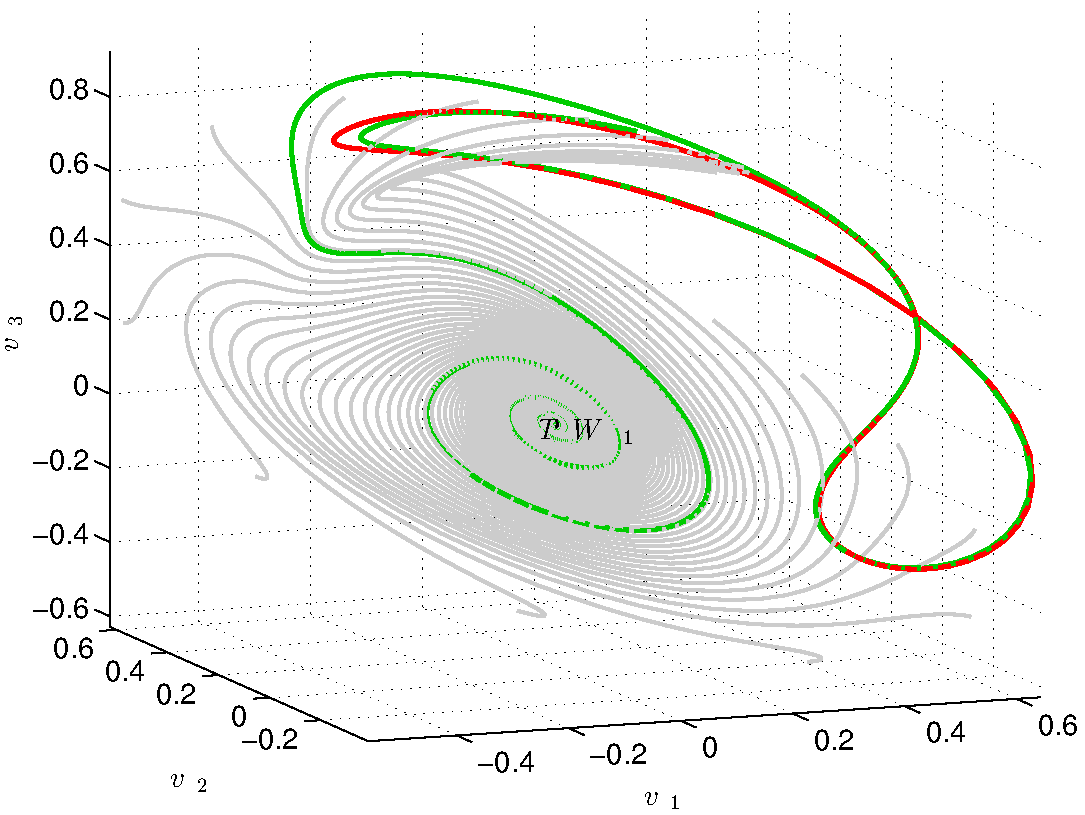
\includegraphics[width=0.45\textwidth]{ks22_TW1_manif_inv_shad_RPO_1631}
 \end{center}
\caption{\label{f:ks22_TW1_manifold}
(a) Unstable manifold of \REQV{-}{1} in $m=2$ slice (grey), \RPO{16.31} (red)
and orbit (green) on unstable manifold of \REQV{-}{1} shadowing \RPO{16.31},
indicating a possible heteroclinic connection.
The coordinate axes $v_1$, $v_2$, and $v_3$ are constructed from 
vectors Re\,$\jEigvec[1]$,
Im\,$\jEigvec[1]$, and Re\,$\jEigvec[3]$ by Gram-Schmidt orthogonalization.
  }
\end{figure*}

Different parts of the unstable submanifold of \REQV{}{1}
corresponding to the leading expanding pair of complex eigenvalues
projected on variables \refeq{eq:SO2polarExt}.
(in the full state space) and transformed to reduced space through
transformations \refeq{eq:SO2polarExt}. (a) Trajectories on the unstable
manifold of \REQV{}{1} (red) which come to the neighborhood of $\EQV{2}$.
Those which come closest to $\EQV{2}$ leave its neighborhood tracing its
unstable manifold (shown in light blue). (b) Nonlinear folding of
trajectories on the unstable manifold of \REQV{}{1} (black) appears
related to the existence of \rpo s of \reffig{f:rpo_shad}. However, it is
more efficient to use the manifolds of the shortest orbits to study the
corresponding return maps.

\section{Conclusions}


\begin{acknowledgments}
\end{acknowledgments}

\appendix



%% Note: Multiple references in a single citation supported using
%% starred (*) argument to the \cite command.
\bibliography{../bibtex/siminos}

                \ifdraft\newpage
\section{Deep freeze\label{c-freeze}}
\input ../blog/freeze.tex
                \fi

\end{document}
